In this chapter, our aim is to introduce some of the fundamental concepts and ideas underlying the proof of the $\ell^2$-decoupling in the two-dimensional case.
Our presentation draws heavily from sources, including the original work by Bourgain and Demeter [BD14], and the most recent proof for the parabola which can be seen as a particular case of [Short Proof].

On the first half of this chapter we present what is known as the bilinear Reduction which allows us to transform our problem into a multilinear one, this observation is the first major driving force of the proof and here we follow a curated 
version of the original work, see [DEM17]. For the later half we present some techniques used in [Short Proof] resorting to some heuristics of the Fourier transform which allows us to see the second driving force of the proof from a geometrical 
perspective, this is the content of subsections \ref{subsection:Wave packet approach} and \ref{subsection:Averaging approach}.

The choice to deviate from the original work is two-fold. Following [BD14], the analogous version of subsection \ref{section:bootstrap} isn't that more complicated, however since we are interested in proving the analogous problem for the moment 
curve this approach won't accomplish that, so this nicely sets up the work for Chapter 2 and allows us to more easily see the geometric aspect of the decoupling problems.

\newpage
\section{Parabola} 
Consider the subset of the parabola above $[0,1]$, parameterized in the usual way, $$\Gamma(t)=(t,t^2)\text{, }t\in[0,1].$$ For $\delta \in (0,1)$, let $\Part(\delta)$ denote the partition of the interval $[0,1]$ into dyadic intervals with length $2^{-\lceil \log_2 \delta^{-1} \rceil}$.
For a dyadic interval $J$, let $\calU_{J}$ be the parallelepiped of dimensions $\abs{J}^{1} \times \abs{J}^{2}$ whose center is $\Gamma(c_J)$ and sides are parallel to $\partial^{1}\Gamma(c_{J})$, $\partial^{2}\Gamma(c_{J})$, where $c_J$ is the center of $J$.
We write $\norm{\cdot}_{6} := \norm{\cdot}_{L^{6}(\R^{2})}$.
\begin{center}
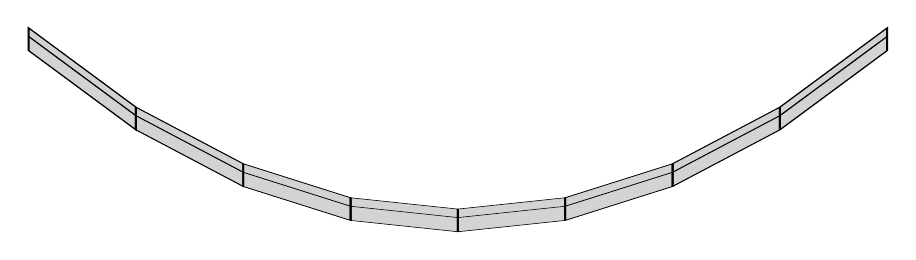
\begin{tikzpicture}[scale=0.5,xscale=3.5]

\definecolor{darkgray176}{RGB}{176,176,176}
\definecolor{lightgray}{RGB}{211,211,211}

\begin{axis}[
hide x axis,
hide y axis,
tick align=outside,
tick pos=left,
x grid style={darkgray176},
xmin=-1.1, xmax=1.1,
xtick style={color=black},
y grid style={darkgray176},
ymin=-0.134375, ymax=1.103125,
ytick style={color=black}
]
\path [draw=lightgray, fill=lightgray]
(axis cs:-1,0.921875)
--(axis cs:-0.75,0.484375)
--(axis cs:-0.75,0.609375)
--(axis cs:-1,1.046875)
--cycle;
\path [draw=lightgray, fill=lightgray]
(axis cs:-0.75,0.484375)
--(axis cs:-0.5,0.171875)
--(axis cs:-0.5,0.296875)
--(axis cs:-0.75,0.609375)
--cycle;
\path [draw=lightgray, fill=lightgray]
(axis cs:-0.5,0.171875)
--(axis cs:-0.25,-0.015625)
--(axis cs:-0.25,0.109375)
--(axis cs:-0.5,0.296875)
--cycle;
\path [draw=lightgray, fill=lightgray]
(axis cs:-0.25,-0.015625)
--(axis cs:0,-0.078125)
--(axis cs:0,0.046875)
--(axis cs:-0.25,0.109375)
--cycle;
\path [draw=lightgray, fill=lightgray]
(axis cs:0,-0.078125)
--(axis cs:0.25,-0.015625)
--(axis cs:0.25,0.109375)
--(axis cs:0,0.046875)
--cycle;
\path [draw=lightgray, fill=lightgray]
(axis cs:0.25,-0.015625)
--(axis cs:0.5,0.171875)
--(axis cs:0.5,0.296875)
--(axis cs:0.25,0.109375)
--cycle;
\path [draw=lightgray, fill=lightgray]
(axis cs:0.5,0.171875)
--(axis cs:0.75,0.484375)
--(axis cs:0.75,0.609375)
--(axis cs:0.5,0.296875)
--cycle;
\path [draw=lightgray, fill=lightgray]
(axis cs:0.75,0.484375)
--(axis cs:1,0.921875)
--(axis cs:1,1.046875)
--(axis cs:0.75,0.609375)
--cycle;
\addplot [line width=0.4pt, black]
table {%
-1 1
-0.75 0.5625
-0.5 0.25
-0.25 0.0625
0 0
0.25 0.0625
0.5 0.25
0.75 0.5625
1 1
};
\addplot [line width=0.4pt, black]
table {%
-1 0.921875
-0.75 0.484375
-0.75 0.609375
-1 1.046875
-1 0.921875
};
\addplot [line width=0.4pt, black]
table {%
-0.75 0.484375
-0.5 0.171875
-0.5 0.296875
-0.75 0.609375
-0.75 0.484375
};
\addplot [line width=0.4pt, black]
table {%
-0.5 0.171875
-0.25 -0.015625
-0.25 0.109375
-0.5 0.296875
-0.5 0.171875
};
\addplot [line width=0.4pt, black]
table {%
-0.25 -0.015625
0 -0.078125
0 0.046875
-0.25 0.109375
-0.25 -0.015625
};
\addplot [line width=0.4pt, black]
table {%
0 -0.078125
0.25 -0.015625
0.25 0.109375
0 0.046875
0 -0.078125
};
\addplot [line width=0.4pt, black]
table {%
0.25 -0.015625
0.5 0.171875
0.5 0.296875
0.25 0.109375
0.25 -0.015625
};
\addplot [line width=0.4pt, black]
table {%
0.5 0.171875
0.75 0.484375
0.75 0.609375
0.5 0.296875
0.5 0.171875
};
\addplot [line width=0.4pt, black]
table {%
0.75 0.484375
1 0.921875
1 1.046875
0.75 0.609375
0.75 0.484375
};
\end{axis}

\end{tikzpicture}
\end{center}
\begin{defn}\label{def:dec-const}
For $\delta \in (0,1)$, the \emph{$\ell^{2}L^{6}$ decoupling constant} $\Dec(\delta)$ for the parabola is the smallest number for which the inequality
\begin{equation}
\label{eq:dec-const}
\norm{ \sum_{J \in \Part(\delta)} f_{J} }_{p_{k}}
\leq \Dec(\delta)
\Bigl( \sum_{J \in \Part(\delta)} \norm{ f_{J} }_{p_{k}}^{2} \Bigr)^{1/2}
\end{equation}
holds for any tuple of functions $(f_{J})_{J \in \Part(\delta)}$ with $\text{supp} \widehat{f_{J}} \subseteq \calU_{J}$ for all $J$.
\end{defn}

\begin{thm}[BD14]\label{thm:main}
For every $\epsilon>0$, there exists a finite constant $C_{\epsilon}$ such that
\begin{equation}
\label{eq:main}
\Dec(\delta) \le C_{\epsilon} \delta^{-\epsilon}, \text{ for every } \delta\in (0, 1).
\end{equation}
\end{thm}


In the original work, the authors proved Theorem \ref{thm:main} by working with a slightly different geometry in the frequency domain. They considered a $\delta^2$-neighborhood of the parabola, denoted by $\mathcal{N}(\delta)\defeq \{(t,t^2+s)\mid t\in[0,1], s\in[0,\delta^2]\}$, partitioned it into almost rectangular boxes $\theta_{J}\defeq\{(t,t^2+s)\mid t\in J, s\in[0,\delta^2]\}$ and considered $(f_{J})_{J \in \Part(\delta)}$ with $\text{supp} \widehat{f_{J}} \subseteq \theta_{J}$ for all $J$ in Definition \ref{def:dec-const}. Let's call $\mathfrak{D}(\delta)$ the \emph{$\ell^{2}L^{6}$} decoupling constant for the curved partition.

We can easily see $\mathfrak{D}(\delta)\lesssim \Dec(\delta)$ by the following picture,
\begin{center}
\begin{tikzpicture}[scale=2]
\begin{axis}[
    hide axis,
    enlarge x limits=0.8, % Add horizontal margin
    enlarge y limits=0.8  % Add vertical margin
    ]

% Plot 1
\addplot [name path = A,
    domain = 0:0.45] {x^2+0.1};

% Plot 2
\addplot [name path = B,
    domain = 0:0.45] {x^2};

 %plot3
\addplot [name path = C,
    domain = 0:0.45] {x^2-0.1};

\addplot [black!20] fill between [of = A and C, soft clip={domain=0:0.45}];

%draw left points of parallelogram
\draw (0,-0.1-0.05) -- (0,0.1);

%draw right points of parallelogram
\draw (0.45,0.45^2+0.1) -- (0.45,0.45^2-0.1-0.05);

\draw (0,-0.1-0.05) -- (0.45,0.45^2-0.1-0.05);
\draw (0,0.1) -- (0.45,0.45^2+0.1);

% Add curly brackets for side lengths
\draw[decorate,decoration={brace,amplitude=5pt,mirror}] (0,-0.1-0.08) -- node[below=6pt] {$\sim \delta$} (0.45,0.45^2-0.1-0.08);
\draw[decorate,decoration={brace,amplitude=5pt}] (0.47,0.45^2+0.1) -- node[right=6pt] {$\sim \delta^2$} (0.47,0.45^2-0.1-0.05);

\draw[dashed] (0,-0.1-0.05) -- (0,-0.3); % Starting at (0,-0.1-0.05)
\draw[dashed] (0.45,0.45^2-0.1-0.05) -- (0.45,-0.3); % Starting at 
% Add the bold, thicker, labeled line "I" at the center
\draw[thick, |-|] (0-0.005,-0.3) -- node[below=8pt] {$J$} (0.45+0.005,-0.3);

\end{axis}
\end{tikzpicture}
\end{center}

 Working with this weaker condition is also motivated by the higher-dimensional case where this kind of anisotropic box works well under certain changes of variables.

A crucial component underlining all decoupling proof is the idea that we can rescale the problem and preserve the decoupling property. In the context of the parabola, this idea starts with following observation, let $I =\left[a,a+\eta \right]$ and let $A_I: \mathbb{R}^2 \longrightarrow \mathbb{R}^2$, defined by 

$$
A_I(x_1,x_2) = \begin{pmatrix}
a \\
a^2
\end{pmatrix} +
\begin{pmatrix}
\eta & 0 \\
2a\eta & \eta^2
\end{pmatrix} 
\begin{pmatrix}
x_1 \\
x_2
\end{pmatrix}
$$
then $A_I \Gamma(t)= \Gamma(a+t\eta)$ for $t\in\R$, in particular one maps $\Gamma(I)$ to the whole curve via $A_I^{-1}$. Furthermore, this map preserves the geometry of the frequency space, i.e, for dyadic intervals $I,J$ with $J \subseteq I \subseteq [0,1]$, we have
\[
A_I^{-1} \calU_{J} = \calU_{J_I},
\]
where $J_I := \eta^{-1} (J - a)$ if $I = [a,a+\eta]$. To see why this is true, combine the relation
$$
(DA_I) \partial^i \Gamma(t) = \kappa^i (\partial^i \Gamma)(a+t\kappa) \quad \text{for all $i\geq 1$ and $t\in\R$}
$$
with the definition of $\calU_J$ (an exemple calculation is done for the full moment curve).
\begin{lem}(Monotony of decoupling constant)
Given $0<\delta_L \leq \delta_S \leq 1$, $\Dec(\delta_L)\leq \Dec(\delta_S)$.
\end{lem}
\begin{proof}
\begin{equation}
    \sum_{J \in \Part(I,\delta_L)} \norm{ f_{J} }_{6}^{2} = \sum_{J \in \Part(I,\delta_L)}\sum_{J^{\prime} \in \Part(J,\delta_S)} \norm{ f_{J^{\prime}} }_{6}^{2},
\end{equation}
apply $\ell^2(\Part(J,\delta_S)) \leq \#\Part(J,\delta_S)\, \ell^6(\Part(J,\delta_S))$ and sum to obtain
\begin{equation}\label{eq:monotony }
    \lesssim \delta_S ^{1-\frac{1}{3}}\sum_{J \in \Part(I,\delta_L)} \norm{ f_{J^{\prime}} }_{6}^{2} \leq \sum_{J \in \Part(I,\delta_L)} \norm{ f_{J^{\prime}} }_{6}^{2}.
\end{equation}
Combine \ref{eq:monotony } with Definition \ref{defn:dec-const} to get the desired conclusion.
\end{proof}
\begin{lem}(Parabolic rescaling) \label{lem:lin_rescale}
Let $I \in \Part(2^{-n})$ for some integer $n \geq 0$.
For any $\delta \in (0,2^{-n})$ and any tuple of functions $(f_J)_{J \in \Part(I,\delta)}$ with $\supp  \widehat{f_J} \subseteq \calU_{J}$ for all $J$, the following inequality holds:
\begin{equation} \label{eq:lin_rescale}
\norm{ f_{I} }_{6}
\leq
\Dec(2^{n} \delta) \Bigl( \sum_{J \in \Part(I, \delta)} \norm{ f_{J} }_{6}^{2} \Bigr)^{1/2}.
\end{equation}
\end{lem}
\begin{proof}
    Suppose that $I = [a,a+2^{-n}]$. For $J \in \Part(I, \delta)$ and $K = J_{I}\in \Part(2^{n}\delta)$, let the function $g_{K}$ be such that  $\widehat{f_{J}} \circ A_{I} = \widehat{g_{K}}$, so that $\supp\,\widehat{g_{K}} \subseteq \calU_{K}=\calU_{J_{I}}$. Applying \ref{eq:dec-const} to the family $(g_{K})$ and changing variables on both sides we obtain \ref{eq:lin_rescale}.
\end{proof}
There's a couple of observation worth noting about this Lemma. Of course one could formulate the analogous decoupling problem for function Fourier supported in $\calU_{I}$, with decoupling constant denoted by $\Dec_{I}(\delta)$. Trivially we could apply Definition \ref{def:dec-const} to the family $(f_J)_{J \in \Part(I,\delta)}$ and obtain
\begin{equation}
\norm{ f_{I} }_{6}
\leq \Dec(\delta)
\Bigl( \sum_{J \in \Part(I,\delta)} \norm{ f_{J} }_{6}^{2} \Bigr)^{1/2}
\end{equation}
which implies $\Dec_{I}(\delta)\leq \Dec(\delta)$. On another hand, Lemma \ref{lem:lin_rescale} implies $\Dec_{I}(\delta)\leq \Dec(2^{n}\delta)$, which can be seen as a stronger bound since, $\Dec(2^{n}\delta)\lesssim \Dec(\delta)$, by monotony. 

\begin{rmk}(Cost of decoupling)
    We can interpret $\Dec(\delta)$ as the cost of decoupling $[0,1]$ into intervals of size $\delta$, \ref{eq:lin_rescale} tells us that the cost of the decoupling $I$ into intervals of size $\delta$, and easier problem, is $\Dec(2^{n} \delta)$. 
\end{rmk}
As an immediate application of parabolic rescaling we have almost multiplicativity of the decoupling constant.

\begin{lem}(Almost multiplicativity)\label{lem:submulti}
    Let $n\in\N$ and $0<\delta<2^{-n}$, then
    $$
    \Dec(\delta) \leq \Dec(2^{-n})\Dec(2^{n}\delta)
    $$
\end{lem}
\begin{proof}
    By applying decoupling at scale $2^{-n}$ we get,
    $$
    \norm{ f }_{6}
\leq
\Dec(2^{-n}) \Bigl( \sum_{J \in \Part(I, \delta)} \norm{ f_{J} }_{6}^{2} \Bigr)^{1/2}.
    $$
    For each $J\in\Part(I, \delta)$ we apply parabolic rescaling to get,
    $$
    \norm{ f_{I} }_{6}
\leq \Dec(\delta)
\Bigl( \sum_{J \in \Part(I,\delta)} \norm{ f_{J} }_{6}^{2} \Bigr)^{1/2}.
    $$
Combining both equation yields the desired results
$$
\norm{ f }_{6}
\leq
\Dec(2^{-n})\Dec(2^{n}\delta) \Bigl( \sum_{J \in \Part(I, \delta)} \norm{ f_{J} }_{6}^{2} \Bigr)^{1/2}.
$$
\end{proof}

By using Lemma \ref{lem:submulti} we can give a fake proof of Theorem \ref{thm:main}. Let $N\in\N$, and take $\delta=2^{-N}$, then by \ref{lem:submulti}
\begin{equation}\label{base iteration}
\Dec(2^{-N})\leq \Dec(2^{-N+1})\Dec(1/2).
\end{equation}
By applying relation \ref{base iteration} $N-1$  times we get the bound
\begin{equation}
\Dec(2^{-N}) \leq \Dec(1/2)^N
\end{equation}
so it's enough to show Theorem \ref{eq:main} at scale $1/2$.
To see why this is true, restrict $1/2\leq \delta_0<1$ and use Cauchy-Schwartz, $\Dec(\delta_0)\leq \delta_0^{-1/2}$, to conclude $\Dec(\delta_0) \lesssim 1$. Plugging this into \ref{base iteration}, $$\Dec(2^{-N}) \leq C^N \text{, for some } C>0.$$
Alternative, for $1/2\leq \delta_0 <1$, there exists a $C_\varepsilon>0$ such that $\Dec(\delta_0)\leq C_\varepsilon\delta_{0}^{-\varepsilon}$, so  $$\Dec(\delta)\leq C_{\varepsilon}^{N} \delta^{-\varepsilon}.$$ Both conclusions reach the same problem: we cannot adequately control the constant. 

Of course, things aren't this easy and the above proof can't be fixed, however, it highlights the idea of induction on scales so prevalent on decoupling proofs. Inequalities in the spirit of \ref{base iteration} to move the problem to a bigger scale at the cost of a factor which can be controlled by the induction hypothesis, Cauchy-Schwartz for a compact range of large scales. 


\section{Biliner-to-linear reduction}
Based on the the fake proof we can infer that a induction on scales procedure might be fruitful, however $\Dec(\delta)$ might not be the appropriated object apply this strategy. Desirably one would find an alternative object, possibly more complicated with extra parameters,  related it to the original problem and prove some property in the spirit of almost multiplicity for which an induction on scales can be effectively employed. There isn't a systematic approach on choosing this objects, but we will start by analysing a bilinear one, which in this two dimensional setting can be seen as natural generalisation. 


\begin{defn}\label{def:bilinear decoupling}
For $\delta \in (0,1/4)$, the bilinear decoupling constant $\BilinDec(\delta)$ for the parabola, is the smallest constant such that, for any pair of intervals $I,I' \in \Part(1/4)$ with $\dist(I,I') \geq 1/4$ and any tuple of functions $(f_{J})_{J \in \Part(I,\delta) \cup \Part(I',\delta)}$ with $\supp \widehat{f_{J}} \subseteq \calU_{J}$ for all $J$, the following inequality holds:
\begin{equation}
\label{eq:BilinDec}
\int_{\R^k} \abs{f_{I}}^{3} \abs{f_{I'}}^{3} \leq
\BilinDec(\delta)^{6} \Bigl(\sum_{J \in \Part(I,\delta)} \norm{f_J }_{6}^2 \Bigr)^{6/4}
\Bigl( \sum_{J' \in \Part(I',\delta)} \norm{f_{J'} }_{6}^2 \Bigr)^{6/4}.
\end{equation}   
\end{defn}

Of course, by Cauchy-Schwartz regular linear decoupling control bilinear, $\BilinDec(\delta)\leq \Dec(\delta)$, but we are seeking the reverse inequality, i.e, we want an equivalence between linear and bilinear decoupling. This is, in fact, motivated by the separation condition. By considering $f_I$ and $f_{I'}$ to be of Knapp type, the curvature of the parabola implies that the dual boxes are transversal. Since this intersection is small, there is a big potential for extra cancellation to occur.

\begin{center}
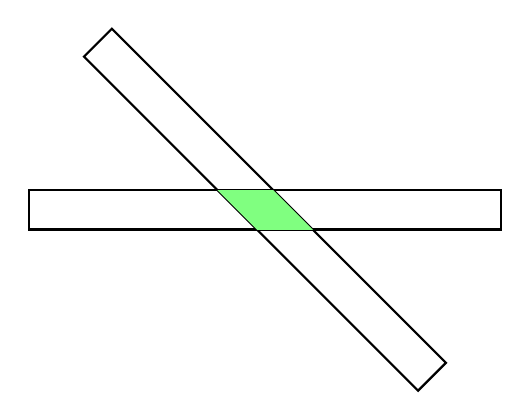
\begin{tikzpicture}
    % Draw first tube
    \draw[thick] (0,0) rectangle (6,0.5);
    % Draw second tube
    \draw[thick,rotate around={-45:(3,0.25)}] (0,0) rectangle (6,0.5);
    % Draw intersection area
    \begin{scope}
        \clip (0,0) rectangle (6,0.5);
        \fill[green!50,rotate around={-45:(3,0.25)}] (0,0) rectangle (6,0.5);
    \end{scope}
\end{tikzpicture}
\end{center}
We won't be able to show a direct equivalence since our methods accumulate logarithmic losses, but we can still achieve a pseudo-equivalence, which is quantified as follows: If $\delta=2^{-N}$, then
\begin{align*}
\Dec(\delta)\lesssim_\e \delta^{-\e}\BilinDec(\delta).
\end{align*}


We can also extend parabolic rescaling to the bilinear setting.

\begin{lem}\label{lem:bilinear parabolic}
Let $I$, $I' \in \Part(2^{-n})$ for some integer $n \geq 2$ such that $2^{-m}\leq\dist(I,I')<2^{-m+1}$ for some $m\leq n$.
For any $\delta \in (0,2^{-n})$ and any tuple of functions $(f_J)_{J \in \Part(I,\delta) \cup \Part(I',\delta})$ with $\supp \widehat{f_J} \subseteq \calU_{J}$ for all $J$, the following inequality holds:
\begin{equation} \label{eq:bilin_rescale}
\int_{\R^2} \abs{f_{I}}^{3} \abs{f_{I'}}^{3} \leq
\BilinDec(2^{m-2} \delta)^{6} \Bigl[ \sum_{J \in \Part(I,\delta)} \norm{f_J }_{6}^2 \Bigr]^{6/4}
\Bigl[ \sum_{J' \in \Part(I',\delta)} \norm{f_{J'} }_{6}^2 \Bigr]^{6/4}.
\end{equation}
\end{lem}

\begin{proof}
    Adapt the proof of \ref{lem:lin_rescale}
\end{proof}

\begin{lem}(Monotony of bilinear decoupling)
Given $0<\delta_L \leq \delta_S \leq 1$, $\BilinDec(\delta_L)\leq \BilinDec(\delta_S)$.
\end{lem}
\begin{proof}
Follows by Lemma (monotony decoupling).
\end{proof}

Let $M\in 2^\N$ and let $\mathcal{C}_M$ be the partition of $[0,1]$ into subintervals $\alpha$ with length $\frac{1}{M}$ so that $\abs{\mathcal{C}_M}=M$. We will write $\alpha\sim\alpha'$ if $\alpha$ and $\alpha'$ are neighbors of each other, and $\alpha\not\sim\alpha'$ otherwise. Notice that each $\alpha$ has at most $3$ neighbors (including itself). The following lemma provides us with a mechanism to deal with the superposition of waves and may be regarded as a model example of the so-called \textit{broad-narrow analysis}. (Add that the result is from Ciprian) 

\begin{lem}\label{bilinear linear elementary lemma}
There are constants $C$ (independent of $M$) and $C_M$ such that
\begin{align}\label{bilinear basic broad-narrow}
    \abs{\sum_{\alpha\in\mathcal{C}_M}z_\alpha}\leq C\max_{\alpha\in\mathcal{C}_M}\abs{z_\alpha}+C_{M}\max_{\alpha'\not\sim\alpha''}\abs{z_{\alpha'}z_{\alpha''}}^{1/2}
\end{align}
for any set of complex numbers $z_\alpha$ indexed by $\alpha\in\mathcal{C}_M$.
\end{lem}
\begin{proof}
Let $\alpha^*$ be such that $\abs{z_{\alpha^*}}=\max_{\alpha\in\mathcal{C}_M}\abs{z_\alpha}$. Define
\begin{align*}
    S_{big}\defeq \{\alpha\in\mathcal{C}_M \mid \abs{z_\alpha} \geq \frac{\abs{z_{\alpha^*}}}{K} \}
\end{align*}
to pick out the \textit{significant} terms on the left hand side of (\ref{bilinear basic broad-narrow}).

First suppose there exists $\alpha_0\in S_{big}$ such that $\alpha_0\not\sim\alpha^*$, then by definition of $S_{big}$ and the triangle inequality, we have
\begin{align*}
    \abs{z_{\alpha_0}z_{\alpha^*}}^{1/2}\geq\frac{\abs{z_{\alpha^*}}}{M^{1/2}}\geq\frac{\abs{\sum_{\alpha\in\mathcal{C}_M}z_\alpha}}{M^{3/2}},
\end{align*} 
which immediately implies that
\begin{align*}
    \quad\abs{\sum_{\alpha\in\mathcal{C}_M}z_\alpha}\leq M^{3/2}\max_{\alpha'\not\sim\alpha''}\abs{z_{\alpha'}z_{\alpha''}}^{1/2}.
\end{align*}
Hence we can choose $C_{M}=M^{3/2}$ on the right hand side of (\ref{bilinear basic broad-narrow}) to complete the proof.

Otherwise, every cube in $S_{big}$ must lie in the neighbor of $\alpha^*$, so we can dominate the left hand side of (\ref{bilinear basic broad-narrow}) using the triangle inequality:
\begin{align*}
    \abs{\sum_{\alpha\in\mathcal{C}_M}z_\alpha}&\leq\sum_{\alpha\sim\alpha^*}\abs{z_\alpha}+\sum_{\alpha\not\sim\alpha^*}\abs{z_\alpha}\\
    &\leq 3\abs{z_{\alpha^*}}+M\frac{\abs{z_{\alpha^*}}}{M}\\
    &=4\max_{\alpha\in\mathcal{C}_M}\abs{z_{\alpha}}.
\end{align*}
Therefore, we can choose $C=4$ on the right hand side of (\ref{bilinear basic broad-narrow}) to complete the proof.

Hence, in both cases (\ref{bilinear basic broad-narrow}) holds.
\end{proof}
\begin{thm}(Bilinear reduction)\label{thm:bilinear reduction} If $\delta=2^{-N}$, then for $n \leq N$
$$
\Dec(\delta)\leq C\Dec(2^{n}\delta) + C 2^{3n/2} \BilinDec(\delta)
$$
\end{thm}
\begin{proof}
    By using Lemma \ref{bilinear linear elementary lemma} with $K=2^k$, $\mathcal{C}_M = \Part(2^{-n})$, and $z_I = f_I(x)$, we have a pointwise inequality:
\begin{align*}
    \abs{F(x)} \leq 4\max_{I\in \Part(2^{-n})}\abs{f_I(x)} + 2^{3n/2} \max_{\substack{J_1,J_2\in\Part(2^{-n})\\ J_1 \not\sim J_2}} \abs{f_{J_1}(x)f_{J_2}(x)}^{1/2}.
\end{align*}

Taking the $L^6$-norm of both sides on $\R^2$, using the triangle inequality,  completing the sums, and finally using Minkowski's integral inequality, we get:
\begin{align*}
    \norm{F}_{L^6(\R^2)} 
    &\leq 
    4\norm{ \max_{J\in \Part(2^{-n})}\abs{f_J} }_{L^6(\R^2)} + 2^{3n/2} 
    \norm{ \max_{\substack{J_1,J_2\in\Part(2^{-n})\\ J_1 \not\sim J_2}} \abs{f_{J_1} f_{J_2}}^{1/2} }_{L^6(\R^2)}\\
    & \leq
    4\norm{\left(\sum_{J\in\Part(2^{-n})}\abs{f_J }^2\right)^{1/2}}_{L^6(\R^2)}
    +
    2^{3n/2} 
    \norm{ \left[\sum_{\substack{J_1,J_2\in\Part(2^{-n})\\ J_1 \not\sim J_2}} \left(\abs{f_{J_1} f_{J_2}}^{1/2}\right)^2 \right]^{1/2}}_{L^6(\R^2)} \\
    & \leq
    4 \left(\sum_{J\in\Part(2^{-n})}\norm{f_J}_{L^6(\R^2)}^2\right)^{1/2}
    +
    2^{3n/2} 
    \left(\sum_{\substack{J_1,J_2\in\Part(2^{-n})\\ J_1 \not\sim J_2}} \norm{\abs{f_{J_1}f_{J_2}}^{1/2}}_{L^6(\R^2)}^2 \right)^{1/2}.
\end{align*}

The first term is known as the narrow term, while the second is known as the broad term. 

Now, the strategy to bound both terms above is parabolic rescaling. For the first term, we can directly apply parabolic rescaling (Lemma \ref{lem:lin_rescale}),

\begin{align*}
\left(\sum_{J\in\Part(2^{-n})}\norm{f_J}_{L^p(\R^2)}^2\right)^{1/2}
    & \leq
    \Dec(2^{n}\delta) \left( \sum_{J\in\Part(2^{-n})} \sum_{J'\in\Part(J,\delta)} \norm{f_{J'}}_{L^6(\R^2)}^2 \right)^{1/2}\\
    & = \Dec(2^{n}\delta)\left(\sum_{J\in\Part(\delta)}\norm{f_{J'}}_{L^6(\R^2)}^2\right)^{1/2}.
\end{align*}
For the broad term, we observe that if $J_1$, $J_2 \in \Part(2^{-n})$ for some integer $n \geq 2$ and there is some $m\leq n$ such that $2^{-m}\leq\dist(I,I')<2^{-m+1}$, then by applying Lemma \ref{lem:bilinear parabolic} and using the monotonicity of the bilinear decoupling constant, we obtain,
\begin{align*}
    \norm{\abs{f_{J_1}f_{J_2}}^{1/2}}_{L^6(\R^2)}&\leq \BilinDec(2^{m-2}\delta)\left(\sum_{J\in\Part(J_1, \delta)}\norm{f_J}_{L^6(\R^2)}^2\sum_{J\in\Part(J_2, \delta)}\norm{f_J}_{L^6(\R^2)}^2\right)^{1/4}\\
    &\leq\BilinDec(2^{m-2}\delta)\left(\sum_{J\in\Part(\delta)}\norm{f_J}_{L^6(\R^2)}^2\right)^{1/2} \leq \BilinDec(\delta)\left(\sum_{J\in\Part(\delta)}\norm{f_J}_{L^6(\R^2)}^2\right)^{1/2}.
\end{align*}

Therefore, combining the estimates for both terms together, we obtain
\begin{align*}
    \norm{f}_{L^6(\R^2)}\leq \left(C\Dec(2^{n}\delta)+C2^{3n/2}2^{n}\BilinDec(\delta)\right)
    \left(\sum_{J\in\Part(\delta)}\norm{f_J}_{L^6(\R^2)}^2\right)^{1/2}
\end{align*}
which immediately implies that for any $n<N$:
\begin{align*}
    \Dec(\delta)\leq C\Dec(2^{n}\delta)+C_n\BilinDec(\delta).
\end{align*}
\end{proof}

\begin{cor}(Iteration) If $\delta=2^{-N}$, then
 \begin{align*}
    \Dec(\delta)\lesssim_\e \delta^{-\e}\BilinDec(\delta).
\end{align*} 
\end{cor}
\begin{proof}
Now we iterate the above inequality. The first few steps of the iteration looks like:
\begin{align*}
     \Dec(\delta)&\leq C\Dec(2^{-N+n})+C_n\BilinDec(\delta)\\
     &\leq C\left(C\Dec(2^{-N+2n}) + C_n\BilinDec(\delta)\right) + C_k\BilinDec(\delta)\\
     &\leq C^2\Dec(2^{-N+2n})+C_n(C+1)\BilinDec(\delta)
\end{align*}
If we repeat this $\frac{N}{n}$ times, then we would get
\begin{align*}
    \Dec(\delta)&\leq C^{N/n}\on\Dec(2^{-N+2\ceil{\frac{N}{n}}}n)+C_n(C^{N/n-1}+...+C+1)\BilinDec(\delta)\\
    &\lesssim C^{N/n}\left(1+C_n\BilinDec(\delta)\right)
\end{align*}
where we used the fact that $\Dec(2^{-N+2\ceil{\frac{N}{n}}}n)\sim \Dec(1/2) \lesssim1$ and computed the sum of the geometric series.


Finally, to conclude the argument we argue as follows. Fix any $\e>0$. If $N > \frac{\log_2C}{\e}+1$, then taking $k=\ceil{\frac{\log_2C}{\e}}<N$ yields
\begin{align*}
    \Dec(\delta)\lesssim 2^{N\e}\left(1+C_\e\BilinDec(\delta)\right)\lesssim_\e 2^{N\e}\left(1+\BilinDec(\delta)\right).
\end{align*}
On the other hand, if $N\leq\frac{\log_2C}{\e}+1$, then note that we always have the trivial estimate $\Dec(2^{-N})\leq 2^{N/2}$ by the Cauchy-Schwarz inequality, and therefore
\begin{align*}
    \Dec(\delta)\leq 2^{\frac{\log_2C}{2\e}+\frac{1}{2}}\lesssim_\e 1 \leq 2^{n\e}\left(1+\BilinDec(\delta)\right).
\end{align*}
Hence,
\begin{align*}
    \Dec(2^{-N})\lesssim_\e 2^{N\e}\BilinDec(2^{-N}).
\end{align*}
\end{proof}
Observation: we will be able to improve on the result to a log loss.
\newpage
\section{Asymmetric bilinear constant}
At this stage, our exposition diverges from the original Bourgain-Demeter argument [BD14]. We won't work with the bilinear constant itself, but with a similar bilinear object which was initially introduced by Li in []. 
(The full general form is highly inspired by the number-theoretic method known as efficient congruencing, developed by Wooley to prove the Vinogradov mean value theorem, see [Wooley15] or [Lilian Pierce].)

\begin{defn}\label{def>asymmetric bilinear}
For $a,b \in [0,1]$ and $\delta \in (0,1)$, the \emph{(asymmetric) bilinear decoupling constant} $\BilinDec_{a, b}(\delta)$ for the parabola is the smallest constant such that, for all pairs of intervals $I \in \Part(\delta^a)$, $I' \in \Part(\delta^b)$ with $\dist(I, I') \ge 1/4$ and all tuples of functions $(f_{J})_{J \in \Part(I,\delta) \cup \Part(I',\delta)}$ with $\supp \widehat{f_{J}} \subseteq \calU_{J}$ for all $J$, the following inequality holds:

\begin{equation}
\label{eq:asymetric constant}
 \int_{\R^2} \abs{f_{I}}^{2}  \abs{f_{I'}}^{4}
\leq \BilinDec_{a, b}(\delta)^{6}\Bigl( \sum_{J \in \Part(I,\delta)} \norm{f_J }_{6}^2 \Bigr) \Bigl( \sum_{J' \in \Part(I',\delta)} \norm{f_{J'} }_{6}^2 \Bigr)^{2}.
\end{equation}
\end{defn}
By using Hölder's inequality we have $\BilinDec_{a, b}\lesssim \delta^{-1/2}$.

The $\BilinDec_{a, b}$ encodes the cost to decouple two intervals of size $\delta^ a$ and $\delta^b$ respectively into intervals of size $\delta$. 
Informally, by considering \(a = b\) and taking \(a \approx 1\), then \(\delta^a \approx C_{1}\delta\) for some \(C_{1} > 0\), so the cost to decouple both \(I\) and \(I'\) into intervals of size \(\delta\) will be a constant \(C_{2}\). Thus, as in the case of almost multiplicity, it is a desirable property to control \(\BilinDec_{a, b}\) by some decoupling constant at a larger scale.
\newline
In the case of the parabola we can in fact prove the following:

\begin{lem}[White lie 1] \label{lem:b}
Let $\delta \in (0,1)$ and $(f_K)_{K \in \Part(\delta)}$ be a tuple of functions so that $\supp \widehat{f_K} \subset \calU_K$ for every $K$.
If $0 \leq a \leq 2b$, then, for any pair of frequency intervals $I \in \Part(\delta^a)$, $I' \in \Part(\delta^b)$ with $\dist(I,I') \geq 1/4$, we have
\begin{equation}\label{eq:fiber-dec}
    \int_{\R^2}  \abs{f_{I}}^{2}\abs{f_{I'}}^{4} \lesssim \sum_{J\in \Part(I,\delta^{2b})}  \int_{\R^2} \abs{f_{J}}^{p_{l}} \abs{f_{I'}}^{4} .
\end{equation}
\end{lem}
By the definition of asymmetric bilinear decoupling constants this results immediately implies the following:
\begin{thm}\label{thm: key step}
For any $0 \leq a \leq 2b$ and $\delta \in (0,1)$, we have
\[
\BilinDec_{a,b}(\delta)
\lesssim
\BilinDec_{2b, b}(\delta).
\]
\end{thm}

This theorem is a manifestation the the phenomenon described above, we can controller the asymmetric billinear constant, $\BilinDec_{a,b}$, by a decoupling constant at a bigger scale, $\BilinDec_{2b,b}$.\\

To justify the sufficient of only studying the asymetric bilinear constant the following results justifies that:
\begin{lem}
For $a, b \in[0,1]$ and $\delta \in(0,1 / 4)$, we have
\begin{equation*}
\mathcal{B}(\delta) \lesssim \delta^{-a/3 } \delta^{-2b/3} \mathcal{B}_{a, b}(\delta) 
\end{equation*}
\end{lem}

\begin{proof}
     Let $I, I^{\prime} \in \mathcal{P}(1 / 4)$ with $\operatorname{dist}\left(I, I^{\prime}\right) \geqslant 1 / 4$. Let $\left(f_{K}\right)_{K \in \mathcal{P}(I, \delta) \cup \mathcal{P}\left(I^{\prime}, \delta\right)}$ be a tuple of functions with $\operatorname{supp} \widehat{f_{K}} \subseteq \mathcal{U}_{K}$ for all $K$. By Hölder's inequality, we have

\begin{equation*}
\int_{\mathbb{R}^{2}}\left|f_{I}\right|^{3}\left|f_{I^{\prime}}\right|^{3} \leqslant
\left(\int_{\mathbb{R}^{2}}\left|f_{I}\right|^{2}\left|f_{I^{\prime}}\right|^{4}\right)^{1 / 2}\left(\int_{\mathbb{R}^{2}}\left|f_{I}\right|^{4}\left|f_{I^{\prime}}\right|^{2}\right)^{1 / 2} 
\end{equation*}
It suffices to estimate the first term. Again by Hölder's inequality 
\begin{equation}
\int_{\mathbb{R}^{2}}\left|f_{I}\right|^{2}\left|f_{I^{\prime}}\right|^{4}\leqslant \int_{\mathbb{R}^{2}}\left(\sum_{J \in \mathcal{P}\left(I, \delta^{a}\right)}\left|f_{J}\right|\right)^{2}\left(\sum_{J^{\prime} \in \mathcal{P}\left(I^{\prime}, \delta^{b}\right)}\left|f_{J^{\prime}}\right|\right)^{4}
\end{equation}
\begin{equation}
    \leqslant \left|\mathcal{P}\left(I, \delta^{a}\right)\right|^{1}\left|\mathcal{P}\left(I^{\prime}, \delta^{b}\right)\right|^{3} \sum_{J \in \mathcal{P}\left(I, \delta^{a}\right)} \sum_{J^{\prime} \in \mathcal{P}\left(I^{\prime}, \delta^{b}\right)} \int_{\mathbb{R}^{2}}\left|f_{J}\right|^{2}\left|f_{J^{\prime}}\right|^{4}
\end{equation}
By Definition \ref{def>asymmetric bilinear},
\begin{equation}
\int_{\mathbb{R}^{2}}\left|f_{I}\right|^{2}\left|f_{I^{\prime}}\right|^{4} \lesssim \delta^{-a} \delta^{-3b} \mathcal{B}_{a, b}(\delta)^{6}\left[\ell_{K \in \mathcal{P}(I, \delta)}^{2}\left\|f_{K}\right\|_{6}\right]^{2}\left[\ell_{K^{\prime} \in \mathcal{P}\left(I^{\prime}, \delta\right)}^{2}\left\|f_{K^{\prime}}\right\|_{6}\right]^{4}
\end{equation}
\end{proof}

In this section, we won’t provide a rigorous proof for Lemma \ref{lem:b}, which is why we refer to it as a "white lie." For a fully rigorous approach, one would need to formalize our use of the uncertainty principle, see [zane parabola]. However, to focus on presenting the main ideas, delving into this formalization could lead to getting lost in the details.

In the remaining part of the section, we'll show two approaches to achieving such a result. The first approach, in the style of BDG, relying on wave packet decomposition, and the second will be a sketch of the proof by [ShortProof] in the parabola case. We defer these details to the sources, [zane harmonic QP] [video series].
\newline
Common to two approaches, we need a form of decoupling, commonly known as $local$ $L^2$-$orthogonality$.
\begin{lem}[White lie 2]\label{white lie2}
    For $l=1,2$, for $\delta \in (0,1)$, and $B$ be a ball of of a cube in $\R^l$ of radius or side length $\delta^{-l}$. Then,
    \begin{equation}\label{eq:local decoupling}
    || f||_{L^{2}(B)}^{2} \lesssim \sum_{J\in\Part(\delta)} || f_{J}||_{L^{2}(B)} ^{2}
    \end{equation}
\end{lem}
This lemma isn't fully rigorous, since the RHS of \ref{eq:local decoupling} should have a weight instead of a sharp cut-off. (Give a sketch)




\subsection{Wave packet approach}\label{subsection:Wave packet approach}
Take $I,I'  \in \Part(\delta^b)$, with $\dist(I, I') \ge 1/4$. Explain dual box. By the uncertainly principle, $|f_{I}|$ will be essentially constant on translates of the dual box $\freqU_{I}$. Denote as $\mathcal{B}(I)$ the tilling of $\R^2$ by translated copies of $\freqU_{I}$, then it at least morally the following identity is true


\begin{equation}\label{eq: heuristic wave packet}
    |f_{I}| \sim \sum_{T // \, \freqU_{I}} c_{T} 1_{T}.
\end{equation}

To turn this into a true identity we would need the full wave packet decomposition (appendix). 

We can use this decomposition to compute a localize version of the LHS of \ref{eq:BilinDec}. \ref{eq:BilinDec}

\begin{equation}\label{eq:part1 packet}
    \fint_{B(0,\delta^{-2b})} \abs{f_{I}}^{2}  \abs{f_{I'}}^{4} \leq  \sum_{} c_{T}^{2}c_{T^{\prime}}^{4} \frac{|T\cap T^{\prime} |}{|B(0,\delta^{-2b})|} =  \sum_{} c_{T}^{2}c_{T^{\prime}}^{4} \delta ^{2b},
\end{equation}
where in the equality we used the fact that since the intervals are unit separated $T$ and $T'$ will intersected almost orthogonally, so $|T\cap T'|\sim \delta^{-2b}$.

Observe that,
\begin{equation}\label{eq:part2 packet}
     \sum_{} c_{T}^{2}c_{T^{\prime}}^{4} \delta ^{2b} = \sum_{}  c_{T}^{2} \frac{|T|}{|B(0,\delta^{-2b})|} \sum_{}c_{T^{\prime}}^{4} \frac{|T^{\prime}|}{|B(0,\delta^{-2b})|} = \left(\fint_{B(0,\delta^{-2b})}\abs{f_{I}}^{2} \right) \left(\fint_{B(0,\delta^{-2b})}\abs{f_{I^{\prime}}}^{4}   \right).
\end{equation}
Combining \ref{eq:part1 packet} and \ref{eq:part2 packet} yields,

\begin{equation}\label{eq: wave packet local}
\fint_{B(0,\delta^{-2b})} \abs{f_{I}}^{2}  \abs{f_{I'}}^{4}
\leq \left(\fint_{B(0,\delta^{-2b})}\abs{f_{I}}^{2} \right) \left(\fint_{B(0,\delta^{-2b})}\abs{f_{I^{\prime}}}^{4}   \right)
\end{equation}


Now we can apply a local $L^{2}$-orthogonality, i.e, 

\begin{equation}
    \fint_{B(0,\delta^{-2b})}\abs{f_{I}}^{2} \lesssim  \sum_{J\in\Part(I,\delta^{2b})} \fint_{B(0,\delta^{-2b})} |f_{J}|^2.
\end{equation}
By the uncertainly principle, since $|J| = \delta^{2b}$, then $|f_{J}|$ is essentially constant on the dual tube $\mathcal{F}_{J}$, which has dimensions $\delta^{-2b} \times \delta^{-4b}$. Consequently, $B(0,\delta^{-2b})$ is contained in the dual tube, so combining this with \ref{eq: wave packet local} yields

\begin{equation}
    \fint_{B(0,\delta^{-2b})} \abs{f_{I}}^{2}  \abs{f_{I'}}^{4} \lesssim \sum_{J\in\Part(I,\delta^{2b})} \fint_{B(0,\delta^{-2b})} |f_{J}|^2 |f_{I^{\prime}}|^4.
\end{equation}
By introducing a modulation on $f$ we can extend this results to,
\begin{equation}
    \fint_{B} \abs{f_{I}}^{2}  \abs{f_{I'}}^{4} \lesssim \sum_{J\in\Part(I,\delta^{2b})} \fint_{B} |f_{J}|^2 |f_{I^{\prime}}|^4.
\end{equation}
where $B$ is a ball of arbitrary center and radius $\delta^{-2b}$. Since we can tile the plane by a countable family of finite-overlapping balls we get Lemma \ref{lem:b}.


\subsection{Averaging approach/lower dimensional approach}\label{subsection:Averaging approach}
Based on [Lecture 22, Hickman] we can summarized the second approach with the following  
\begin{figure}[h!]
    \centering
    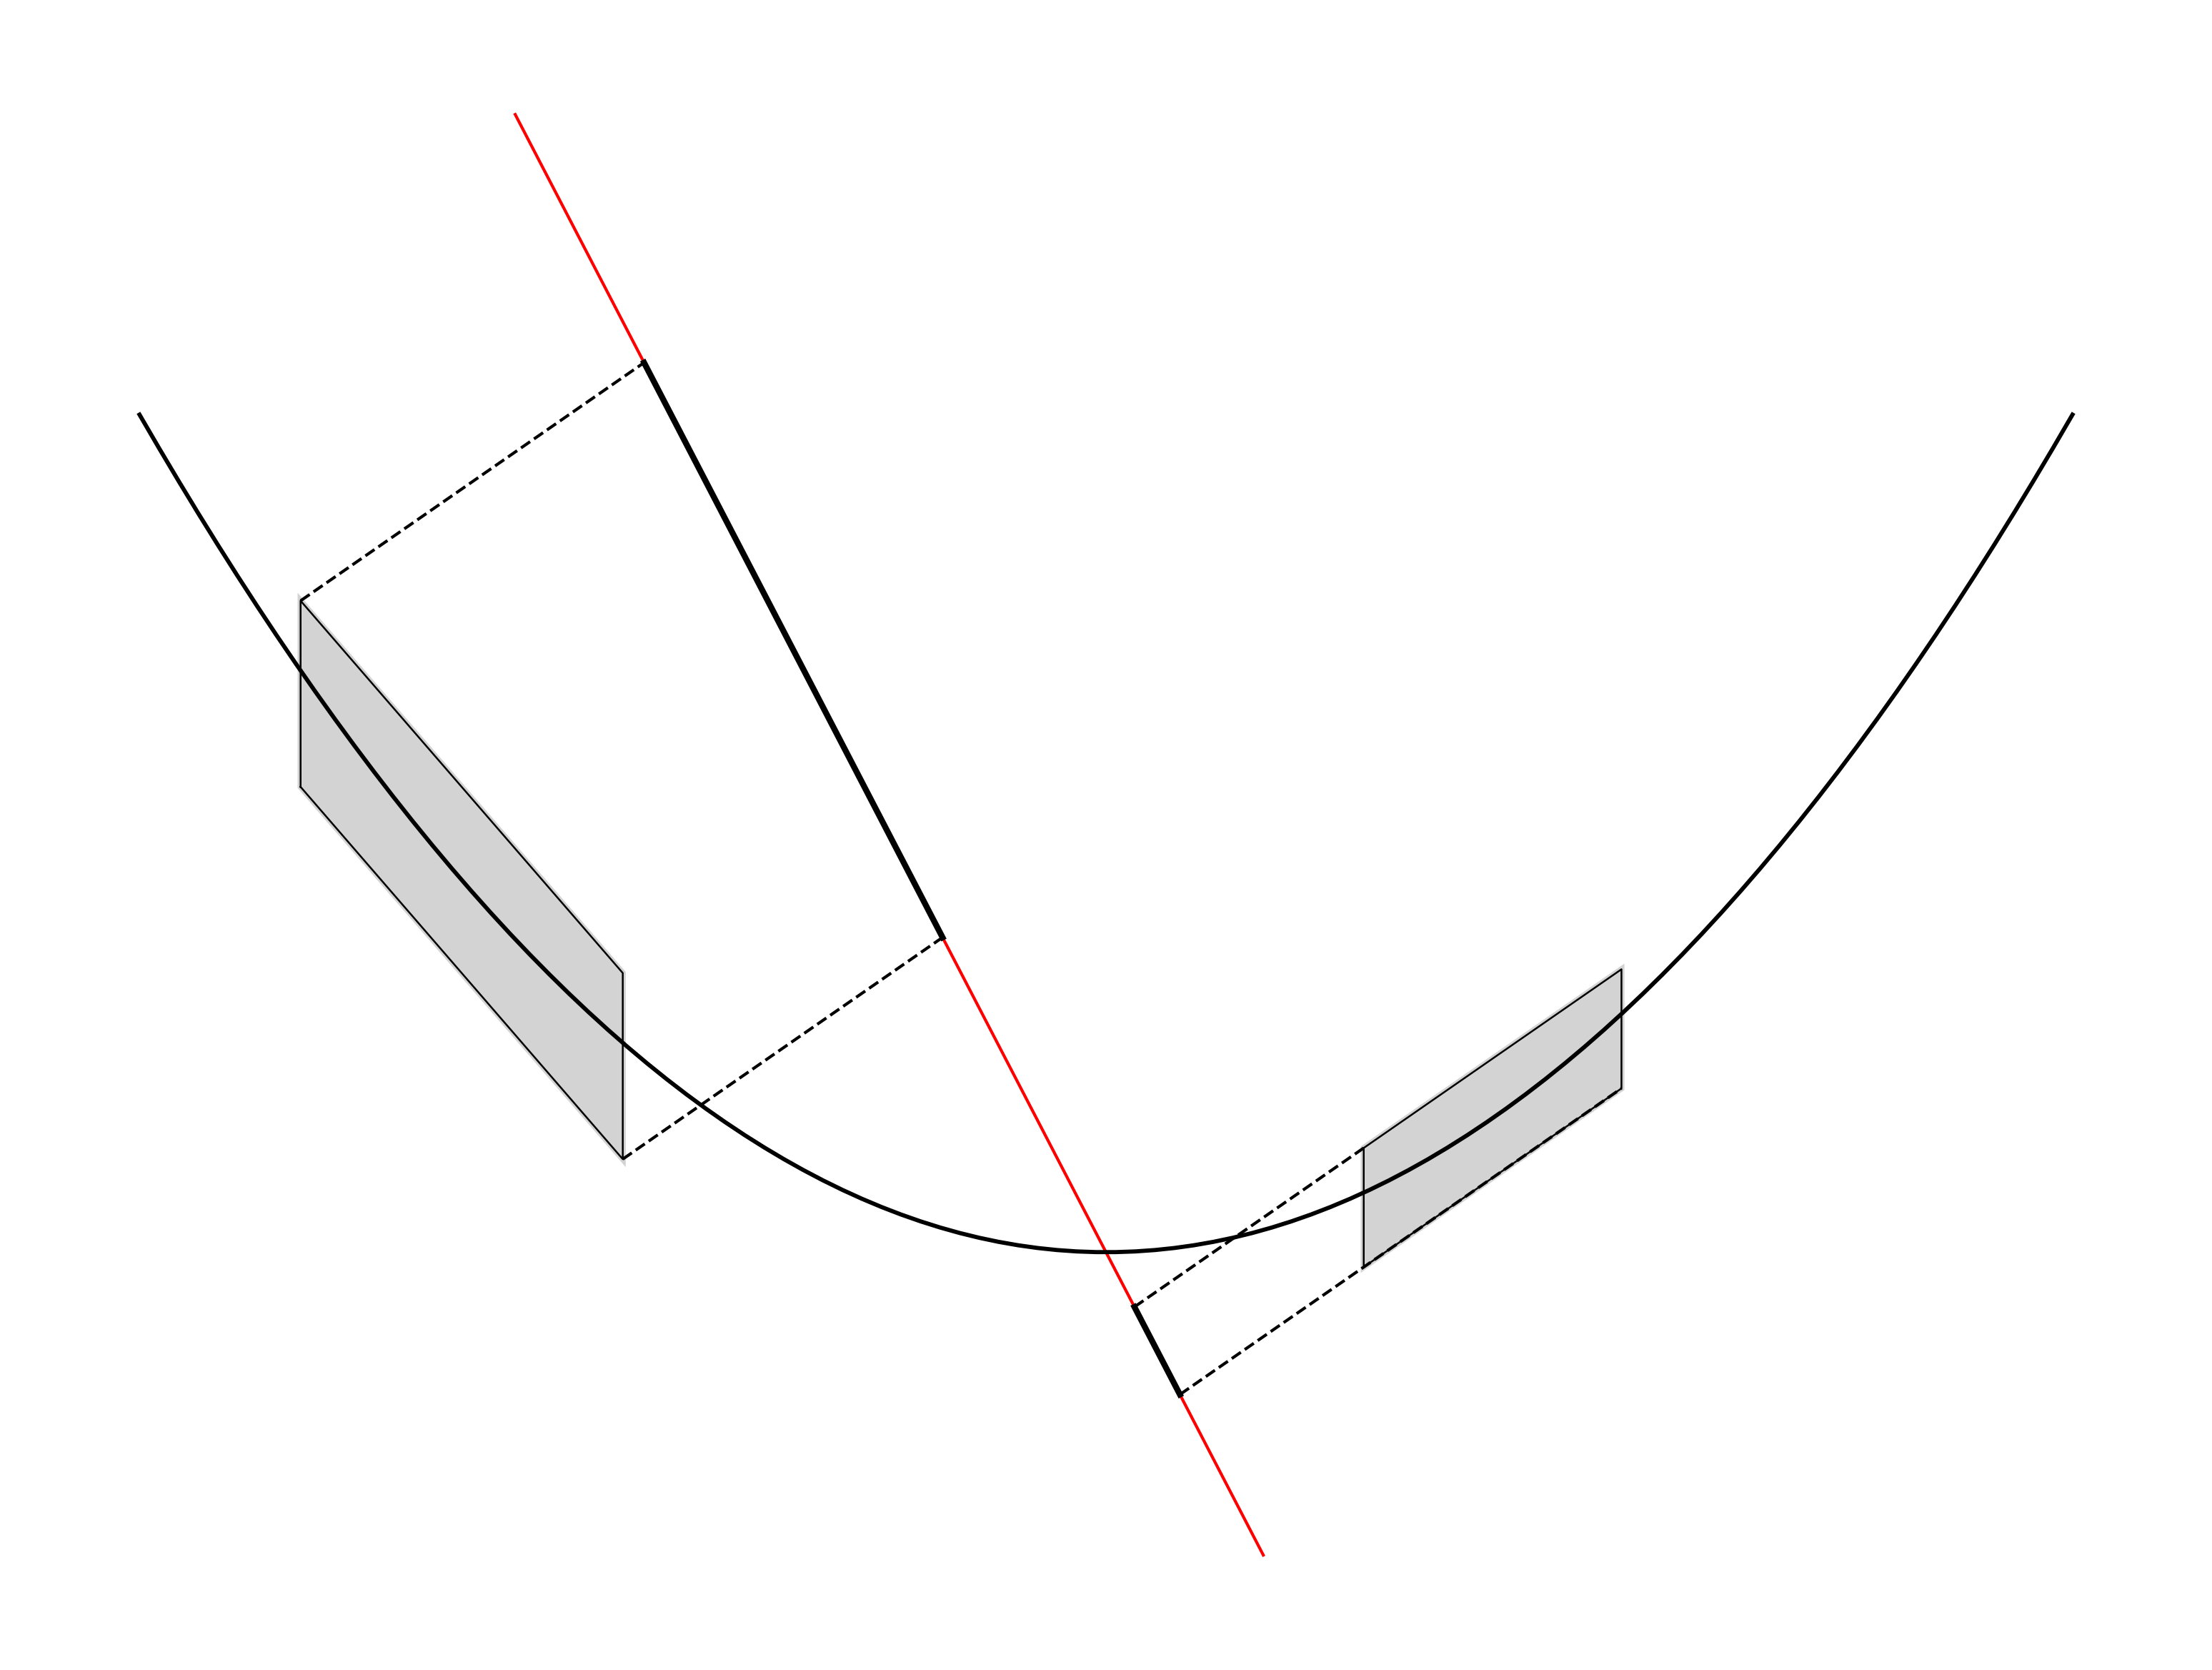
\includegraphics[scale=0.6]{Pics/Proj1.png}
    \caption{Projections }
    \label{fig:projections}
\end{figure}


Consider $I\in \Part(I,\delta^{a})$ and $I^{\prime}\in \Part(I^{\prime},\delta^{b})$, such that $dist(I,I')\geq 1/4$ $\hat{f_{I}}$, $\hat{f_{I^{\prime}}}$ are supported on $\calU_{I}$ and $\calU_{I^{\prime}}$, respectively. Let $\nu:[-1,1]\xrightarrow{}$

For $c_{I^{\prime}}$ define $H = Span\{\nu(c_{I^{\prime}})\}$ to be the subspace of $\R^2$ spanned by $\nu(c_{I^{\prime}})$, see red line in \ref{fig:projections}.

Let $\text{Proj}_{\,H}: \R^{d}\longrightarrow H$, then we have the following geometric consequences,

$$diam(\text{Proj}_{\,H}(\calU_{I^{\prime}}))\lesssim \delta^{2b},$$

in particular we see that $\calU_{I^{\prime}}$ is projects onto a line segment of length $\delta^{2b}$ which corresponds to the shorts side of $\calU_{I^{\prime}}$.

On another hand the unit separation of the intervals translates to a form of tranversality between $\calU_{I}$ and $\calU_{I^{\prime}}$, i.e,
$$
diam(\text{Proj}_{\,H}(\calU_{I}))\sim \delta^{a}
$$
in particular $\calU_{I}$ is projected onto a interval of length $\delta^a$, which corresponds to the long side of $\calU_{I}$.

Now we want to subdivide the interval $I$ into intervals of a smaller scale and then consider what happens to the frequency boxes under this projection map. To make this more precise let $0\leq \eta \leq \delta^ a$, then 

\begin{equation}\label{eq:sub projections}
\{\text{Proj}_{\,H}(\calU_{K}):\, K\in \Part(I,\eta)\}
\end{equation}
is a family of finite-overlapping intervals of length $\sim \eta$.
\begin{figure}[h!]
    \centering
    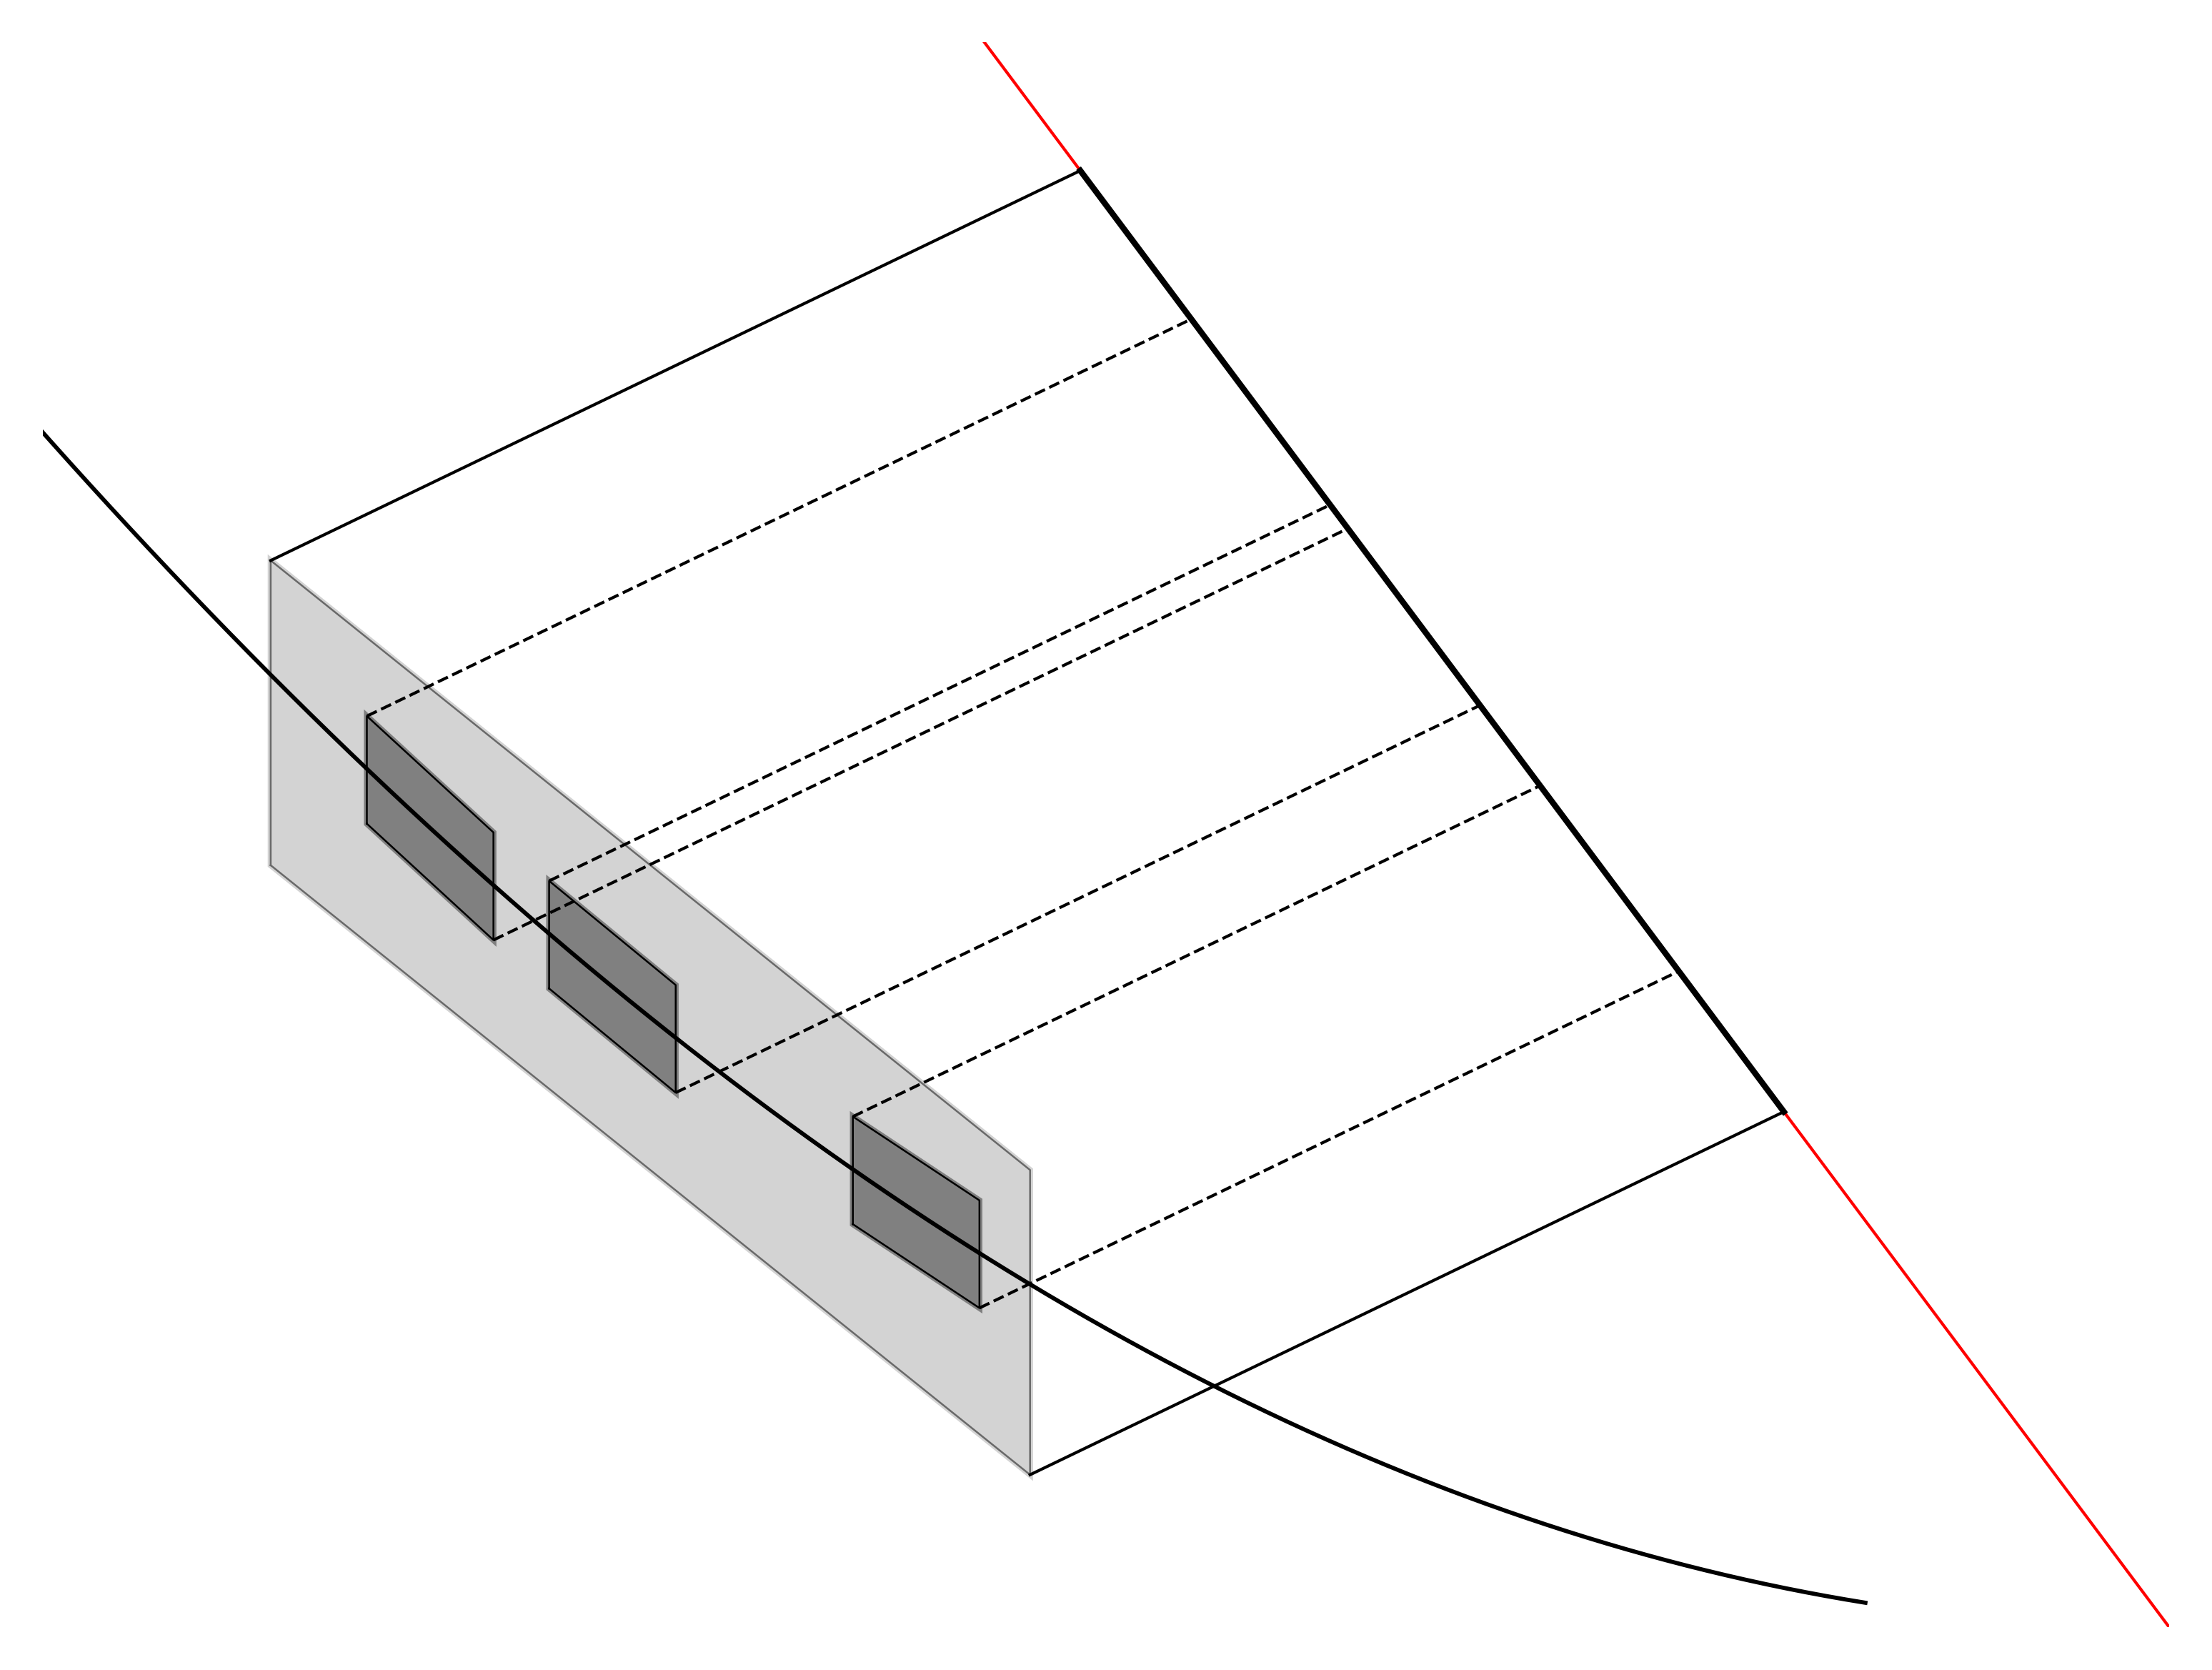
\includegraphics[scale=0.6]{Pics/Proj2.png}
    \caption{Projections}
    \label{fig:projections_overlap}
\end{figure}


To convert all this geometric facts into analytical form, one needs the following auxiliary lemma.
\begin{lem}\label{lem:fourier projecton} 
    Let $f\in \mathcal{S}(\R^d)$ and write $x=(x^{\prime},x^{\prime\prime})\in \R^{k} \times \R^{d-k}$. For each $x^{\prime\prime}$ consider the slice $f_{x^{\prime\prime}}: \R^{k}\longrightarrow \C$ define as $f_{x^{\prime\prime}}(x^{\prime}):=f(x^{\prime},x^{\prime\prime})$,
    then
    $$
    \supp(\, \widehat{f_{x^{\prime\prime}}}) \,\subset \text{Proj}_{\,\R^{k} }(\supp \hat{f})
    $$
    where $\text{Proj}_{\,\R^{k}}: \R^{d}\longrightarrow \R^{k}$; $(\xi^{\prime},\xi^{\prime\prime})\xrightarrow{}\xi^{\prime}$ denotes the orthogonal projection.
\end{lem}
\begin{proof}
    By Fubini's Theorem we can argue,
    \begin{equation}\label{eq:fourier slice}
        \hat{f}(\xi) = \int_{\R^d} f(x^{\prime},x^{\prime\prime}) e(x^{\prime }\cdot \xi^{\prime})e(x^{\prime\prime}\cdot \xi^{\prime})\, dx^{\prime}dx^{\prime\prime} = \int_{\R^{d-k}} (\widehat{f_{x^{\prime\prime}}})(\xi^{\prime})e(x^{\prime\prime}\cdot \xi^{\prime})dx^{\prime\prime} = \mathcal{F}_{x^{\prime\prime}}\left[ \widehat{f_{x^{\prime\prime}}}(\xi^{\prime})\right]
    \end{equation}
    Where $\mathcal{F}_{x^{\prime\prime}} $, denotes the Fourier transform in the $x^{\prime\prime}$ variable.\\
    
    If \(\xi' \not\in \text{Proj}_{\,\R^{k}}(\supp \hat{f})\), then for any \(\xi'' \in \R^{d-k}\), we have \((\xi', \xi'') \not\in \supp \hat{f}\). Therefore, by \eqref{eq:fourier slice}, \(\mathcal{F}_{x''}\left[\widehat{f_{x''}}(\xi')\right] = 0\). Since the Fourier transform is injective, this implies \(\widehat{f_{x''}}(\xi') = 0\). Consequently, \(\xi' \not\in \supp(\widehat{f_{x''}})\).

\end{proof}

From this we see that if we have some function $f_{J}$ in $\mathbb{R}^{2}$ with Fourier support in $\cal{U}_{J}$, then the restriction, $\left.f_{J}\right|_{H}$, of $f_{J}$ to some $1$-dimensional manifold $H$ has its Fourier support contained the projection of $\cal{U}_{J}$ onto $H$.

\begin{lem}
    Let $d\geq 1$ and  $H$ a $k$-dimension linear subspace of $\R^d$. Then by choosing coordinates as in Lemma \ref{lem:fourier projecton},

$$
\int_{\R^2}f =\int_{z\in \R^d}\fint_{B_{H}(x,r)} f
$$
where $B_{H}(x,r)$ is a ball of center $x$ and radius $r>0$, contained in $H$.
\end{lem}
\begin{proof}
    Applying Fubini's Theorem gives

$$
\int_{x\in \R^d}\fint_{B_{H}(x,r)} f = \int_{x\in \R^d} \fint_{B_{\R^2}(0,r)} f(x' + y,x'') \,dy = \fint_{B_{\R^2}}\int_{x\in \R^d} f(x' + y,x'') \,dx\,dy = \int_{x\in \R^d} f.
$$
\end{proof}
Now, we apply this averaging argument to our particular case:
\begin{equation}
\int_{\R^2} \abs{f_{I}}^{2} \abs{f_{I'}}^{4} \,
= \int_{\R^2} \fint_{B_{H}(x,\delta^{-2b})} \abs{f_{I}}^{2} \abs{f_{I'}}^{4} \,.
\end{equation}
By orthogonality, we can argue that $B_{H}(0,\delta^{-2b}) \subseteq \freqU_{I}$ and so, $|f_I|$ is essentially constant on $B_{H}(0,\delta^{-2b})$. Now we apply $L^2$ orthogonality to $\left.f_{I}\right|_{H}$ with radius $\delta^{-2b}$:
$$
\int_{\R^2}\abs{f_{I'}}^{4} \fint_{B_{H}(x,\delta^{-2b})} \abs{f_{I}}^{2}  \, dy \, dx \leq \int_{\R^2}\abs{f_{I'}}^{4} \sum_{J\in\Part(I,\delta^{2b})} || f_{J}||_{L^{2}(B_{H}(x,\delta^{-2b}))} ^{2} = \sum_{J\in\Part(I,\delta^{2b})}\int_{\R^2}|f_{J}|^2\abs{f_{I'}}^{4}.
$$
Observe that the chosen radius is maximal.



\section{Bootstrap}\label{section:bootstrap}
In this section we prove Theorem \ref{thm:main} by using Lemma \ref{thm: key step}.

\begin{lem}[Swap] \label{lem:Hölder}
    If $a, b \in (0,1)$ and $\delta \in (0,1)$, then
\begin{equation}\label{eq:Hölder}
\BilinDec_{a,b}(\delta)
\leq
\BilinDec_{b,a}(\delta)^{\frac{1}{2}} \Dec(\delta^{1-b})^{\frac{1}{2}}.
\end{equation}
\end{lem}
\begin{proof}
By Hölder's inequality,
    \begin{equation}
    \int_{\R^2} |f_I|^2|f_{I^{\prime}}|^4\, dx \leq \left(\int_{\R^2} |f_{I^{\prime}}|^2|f_I|^4\, dx \right)^{\frac{1}{2}}\left(\int_{\R^2}|f_{I}^{\prime}|^6 \, dx \right)^{\frac{1}{2}}.
    \end{equation}

The results follows from the definition of $\BilinDec_{a,b}$ and parabolic rescaling.
\end{proof}

\begin{lem}[Iteration]\label{lem:iteration}
For $b\in [0,1]$ and $b\leq \frac{1}{4}$ we have,
$$
\BilinDec_{2b,b}(\delta) \lesssim (\BilinDec_{4b,2b}(\delta)) ^{\frac{1}{2}}(\Dec(\delta^{1-b})) ^{\frac{1}{2}}
$$  
\end{lem}
\begin{proof}
    Apply Theorem \ref{thm: key step} followed by \ref{lem:Hölder}.
\end{proof}


\begin{proof}[Sketch of Theorem \ref{thm:main}]
Let $\eta$ be the infimum of all $\epsilon$ for which the decoupling inequality \eqref{eq:main} holds.

Define $A_1(b)$ to the the smallest exponent such that 
$$
\BilinDec_{2b,b}(\delta) \lesssim \delta^{-A}
$$
and $A_0(b)$ be the smallest exponent such that

$$
\Dec(\delta^{1-b}) \lesssim \delta ^{-A}.
$$
A direct calculation gives $A_0(b)=\eta(1-b)$.

By applying this definitions to Lemma \ref{lem:iteration},

$$
\BilinDec_{2b,b}(\delta) \lesssim \left[ \delta^{-A_{1}(2b)}\right]^{\frac{1}{2}}\left[ \delta^{-\eta(1-b)}\right]^{\frac{1}{2}}
$$
which can be simplified to 
\begin{equation}\label{eq:iter proof}
A_1(b) \leq A_{1}(2b) + \eta(1-b).
\end{equation}


We extract the information on the asymptotic behaviour of bilinear decoupling exponents $A_{l}(b)$ from the functional inequality \eqref{eq:iter proof} by introducing the quantities
$$
A_{l} := \liminf_{b\to 0} \frac{\eta - A_{l}(b)}{b} \in \R \cup \{\pm\infty\}.
$$

which yields
$$
A_1 \geq A_1 + \frac{1}{2} \eta.
$$

By assuming that $A_1$ is a finite this is equivalent to the claim. (This happens because there is an equivalence between linear and bilinear decoupling)


\end{proof}










































